\chapter{Results}
\label{sec:results}
\section{Training Results}
%TODO: Add training results?

\section{Experiment Results}
\begin{figure}[h!]
	\begin{minipage}{0.5\linewidth}
		\includegraphics[width=\linewidth]{results/exp1/1v1_nodes.pdf}
	\end{minipage}
	
	\begin{minipage}{0.5\linewidth}
		\includegraphics[width=\linewidth]{results/exp2-12k/1v1_nodes.pdf}
	\end{minipage}
	\begin{minipage}{0.5\linewidth}
		\includegraphics[width=\linewidth]{results/exp2-26k/1v1_nodes.pdf}
	\end{minipage}
	
	\begin{minipage}{0.5\linewidth}
		\includegraphics[width=\linewidth]{results/exp3-12k/1v1000_nodes.pdf}
	\end{minipage}
	\begin{minipage}{0.5\linewidth}
		\includegraphics[width=\linewidth]{results/exp3-26k/1v1000_nodes.pdf}
	\end{minipage}
	\caption[ Results: Input feature nodes]{ Results of the experiments 1, 2 and 3 for the feature nodes. \\* Experiment 1 (first row): True distribution (red, dashed) vs Generated distribution (blue, solid) in the case of a network with no input features. \\* Experiment 2 (second row): True distribution (red, dashed) vs Generated distribution (blue, solid) in the case of a conditional network trained for 12000 (left) and 26000 (right) iterations. \\* Experiment 3 (third row): Input feature values for the 25th (red), 50th (green), 75th (blue) percentile vs. the corresponding generated distribution}
	\label{fig:results_nodes}
\end{figure}
\begin{figure}[h!]
	\begin{minipage}{0.5\linewidth}
		\includegraphics[width=\linewidth]{results/exp1/1v1_level_solidity.pdf}
	\end{minipage}
	
	\begin{minipage}{0.5\linewidth}
		\includegraphics[width=\linewidth]{results/exp2-12k/1v1_level_solidity.pdf}
	\end{minipage}
	\begin{minipage}{0.5\linewidth}
		\includegraphics[width=\linewidth]{results/exp2-26k/1v1_level_solidity.pdf}
	\end{minipage}
	
	\begin{minipage}{0.5\linewidth}
		\includegraphics[width=\linewidth]{results/exp3-12k/1v1000_level_solidity.pdf}
	\end{minipage}
	\begin{minipage}{0.5\linewidth}
		\includegraphics[width=\linewidth]{results/exp3-26k/1v1000_level_solidity.pdf}
	\end{minipage}
	\caption[ Results: Input feature level\textunderscore solidity]{ Results of the experiments 1, 2 and 3 for the feature level\textunderscore solidity. \\* Experiment 1 (first row): True distribution (red, dashed) vs Generated distribution (blue, solid) in the case of a network with no input features. \\* Experiment 2 (second row): True distribution (red, dashed) vs Generated distribution (blue, solid) in the case of a conditional network trained for 12000 (left) and 26000 (right) iterations. \\* Experiment 3 (third row): Input feature values for the 25th (red), 50th (green), 75th (blue) percentile vs. the corresponding generated distribution}
	\label{fig:results_level_solidity}
\end{figure}
\begin{figure}[h!]
	\begin{minipage}{0.5\linewidth}
		\includegraphics[width=\linewidth]{results/exp1/1v1_level_equivalent_diameter.pdf}
	\end{minipage}
	
	\begin{minipage}{0.5\linewidth}
		\includegraphics[width=\linewidth]{results/exp2-12k/1v1_level_equivalent_diameter.pdf}
	\end{minipage}
	\begin{minipage}{0.5\linewidth}
		\includegraphics[width=\linewidth]{results/exp2-26k/1v1_level_equivalent_diameter.pdf}
	\end{minipage}
	
	\begin{minipage}{0.5\linewidth}
		\includegraphics[width=\linewidth]{results/exp3-12k/1v1000_level_equivalent_diameter.pdf}
	\end{minipage}
	\begin{minipage}{0.5\linewidth}
		\includegraphics[width=\linewidth]{results/exp3-26k/1v1000_level_equivalent_diameter.pdf}
	\end{minipage}
	\caption[ Results: Input feature level\textunderscore equivalent\textunderscore diameter]{ Results of the experiments 1, 2 and 3 for the feature level\textunderscore equivalent\textunderscore diameter. \\* Experiment 1 (first row): True distribution (red, dashed) vs Generated distribution (blue, solid) in the case of a network with no input features. \\* Experiment 2 (second row): True distribution (red, dashed) vs Generated distribution (blue, solid) in the case of a conditional network trained for 12000 (left) and 26000 (right) iterations. \\* Experiment 3 (third row): Input feature values for the 25th (red), 50th (green), 75th (blue) percentile vs. the corresponding generated distribution}
	\label{fig:results_level_equivalent_diameter}
\end{figure}
\begin{figure}[h!]
	\begin{minipage}{0.5\linewidth}
		\includegraphics[width=\linewidth]{results/exp1/1v1_distmap-skew.pdf}
	\end{minipage}
	
	\begin{minipage}{0.5\linewidth}
		\includegraphics[width=\linewidth]{results/exp2-12k/1v1_distmap-skew.pdf}
	\end{minipage}
	\begin{minipage}{0.5\linewidth}
		\includegraphics[width=\linewidth]{results/exp2-26k/1v1_distmap-skew.pdf}
	\end{minipage}
	
	\begin{minipage}{0.5\linewidth}
		\includegraphics[width=\linewidth]{results/exp3-12k/1v1000_distmap-skew.pdf}
	\end{minipage}
	\begin{minipage}{0.5\linewidth}
		\includegraphics[width=\linewidth]{results/exp3-26k/1v1000_distmap-skew.pdf}
	\end{minipage}
	\caption[ Results: Input feature distmap-skew]{ Results of the experiments 1, 2 and 3 for the feature distmap-skew. \\* Experiment 1 (first row): True distribution (red, dashed) vs Generated distribution (blue, solid) in the case of a network with no input features. \\* Experiment 2 (second row): True distribution (red, dashed) vs Generated distribution (blue, solid) in the case of a conditional network trained for 12000 (left) and 26000 (right) iterations. \\* Experiment 3 (third row): Input feature values for the 25th (red), 50th (green), 75th (blue) percentile vs. the corresponding generated distribution}
	\label{fig:results_distmap-skew}
\end{figure}
\begin{figure}[h!]
	\begin{minipage}{0.5\linewidth}
		\includegraphics[width=\linewidth]{results/exp1/1v1_distmap-kurt.pdf}
	\end{minipage}
	
	\begin{minipage}{0.5\linewidth}
		\includegraphics[width=\linewidth]{results/exp2-12k/1v1_distmap-kurt.pdf}
	\end{minipage}
	\begin{minipage}{0.5\linewidth}
		\includegraphics[width=\linewidth]{results/exp2-26k/1v1_distmap-kurt.pdf}
	\end{minipage}
	
	\begin{minipage}{0.5\linewidth}
		\includegraphics[width=\linewidth]{results/exp3-12k/1v1000_distmap-kurt.pdf}
	\end{minipage}
	\begin{minipage}{0.5\linewidth}
		\includegraphics[width=\linewidth]{results/exp3-26k/1v1000_distmap-kurt.pdf}
	\end{minipage}
	\caption[ Results: Input feature distmap-kurt]{ Results of the experiments 1, 2 and 3 for the feature distmap-kurt. \\* Experiment 1 (first row): True distribution (red, dashed) vs Generated distribution (blue, solid) in the case of a network with no input features. \\* Experiment 2 (second row): True distribution (red, dashed) vs Generated distribution (blue, solid) in the case of a conditional network trained for 12000 (left) and 26000 (right) iterations. \\* Experiment 3 (third row): Input feature values for the 25th (red), 50th (green), 75th (blue) percentile vs. the corresponding generated distribution}
	\label{fig:results_distmap-kurt}
\end{figure}
\begin{figure}[h!]
	\begin{minipage}{0.5\linewidth}
		\includegraphics[width=\linewidth]{results/exp1/1v1_level_minor_axis_length.pdf}
	\end{minipage}
	
	\begin{minipage}{0.5\linewidth}
		\includegraphics[width=\linewidth]{results/exp2-12k/1v1_level_minor_axis_length.pdf}
	\end{minipage}
	\begin{minipage}{0.5\linewidth}
		\includegraphics[width=\linewidth]{results/exp2-26k/1v1_level_minor_axis_length.pdf}
	\end{minipage}
	
	\begin{minipage}{0.5\linewidth}
		\includegraphics[width=\linewidth]{results/exp3-12k/1v1000_level_minor_axis_length.pdf}
	\end{minipage}
	\begin{minipage}{0.5\linewidth}
		\includegraphics[width=\linewidth]{results/exp3-26k/1v1000_level_minor_axis_length.pdf}
	\end{minipage}
	\caption[ Results: Input feature level\textunderscore minor\textunderscore axis\textunderscore length]{ Results of the experiments 1, 2 and 3 for the feature level\textunderscore minor\textunderscore axis\textunderscore length. \\* Experiment 1 (first row): True distribution (red, dashed) vs Generated distribution (blue, solid) in the case of a network with no input features. \\* Experiment 2 (second row): True distribution (red, dashed) vs Generated distribution (blue, solid) in the case of a conditional network trained for 12000 (left) and 26000 (right) iterations. \\* Experiment 3 (third row): Input feature values for the 25th (red), 50th (green), 75th (blue) percentile vs. the corresponding generated distribution}
	\label{fig:results_level_minor_axis_length}
\end{figure}
\begin{figure}[h!]
	\begin{minipage}{0.5\linewidth}
		\includegraphics[width=\linewidth]{results/exp1/1v1_level_major_axis_length.pdf}
	\end{minipage}
	
	\begin{minipage}{0.5\linewidth}
		\includegraphics[width=\linewidth]{results/exp2-12k/1v1_level_major_axis_length.pdf}
	\end{minipage}
	\begin{minipage}{0.5\linewidth}
		\includegraphics[width=\linewidth]{results/exp2-26k/1v1_level_major_axis_length.pdf}
	\end{minipage}
	
	\begin{minipage}{0.5\linewidth}
		\includegraphics[width=\linewidth]{results/exp3-12k/1v1000_level_major_axis_length.pdf}
	\end{minipage}
	\begin{minipage}{0.5\linewidth}
		\includegraphics[width=\linewidth]{results/exp3-26k/1v1000_level_major_axis_length.pdf}
	\end{minipage}
	\caption[ Results: Input feature level\textunderscore major\textunderscore axis\textunderscore length]{ Results of the experiments 1, 2 and 3 for the feature level\textunderscore major\textunderscore axis\textunderscore length. \\* Experiment 1 (first row): True distribution (red, dashed) vs Generated distribution (blue, solid) in the case of a network with no input features. \\* Experiment 2 (second row): True distribution (red, dashed) vs Generated distribution (blue, solid) in the case of a conditional network trained for 12000 (left) and 26000 (right) iterations. \\* Experiment 3 (third row): Input feature values for the 25th (red), 50th (green), 75th (blue) percentile vs. the corresponding generated distribution}
	\label{fig:results_level_major_axis_length}
\end{figure}






\section{Generated Samples}
\section{Summary}